\subsection{What is Projectional Editing?}
\label{section:WhatIsPE}

When talking about projectional editing, we are mostly talking in the domain of Meta-programming.
Usually, when we talk about software development, the programmer or developer creates the program and the user who uses it.
In metaprogramming, we are talking about the development of languages.
Here the developer could refer to both the creator and the user.
We will distinguish these two roles in this paper by referring to the creators of the languages as Language Engineers.
Thus when we refer to developers in this paper, we mean users of the language. 

Traditionally developers write code with text editors or integrated development environments (IDE), which adjust the concrete syntax and allows a parser to create the abstract syntax tree.
A projectional editor, Inverts this relationship, as a developer edits the abstract syntax tree and allows the IDE to project the concrete syntax.

\subsubsection{Parser Based Editing}

A program is defined using text and edited with a text editor in a traditional parser-based development workflow.
A grammar is a definition of a programming language's formal syntactical rules or concrete syntax.
One derives the lexer and parser from the grammar.
The lexer will turn text passed into a text buffer into tokens.
A parser then validates that these tokens, the words of the language, are syntactically correct.
The parser then constructs a concrete syntax tree and an abstract syntax tree (AST).

An AST is a tree structure that represents the semantic meaning of the source code, stripped of all the syntactic details.
The parser will carry out some of the name resolutions needed to ensure that the tree represents the references expressed within the source code.
These references turn the tree into a graph.

Compilers use the AST to do subsequent processing, such as linking, transformation, analysis, and type checking.
Modern IDEs, in the background, also parse the code it is displaying to create an AST to offer relevant coding assistance.
This assistance is appreciated as without IDE help learning the concrete syntax of non-trivial languages is error-prone.
Exploratory programming is laborious if one has to wait until compilation to discover mistakes.

\subsubsection{Projectional Definition}

In the projectional editing paradigm, a semantic model represents the program.
This model requires projectional editing tools to be read and edited.

A projectional editor does not parse any text.
In its place, a developer reads and edits a representation of the AST through a projected notation.
Her editing gestures immediately and directly manipulate the AST.
This editing takes place within predefined and fixed templates called editors.

The principle of projectional editing is familiar to those that use visual programming, like Scratch or Blockly, or graphical modelling tools, such as MetaEdit+.
These tools do not parse pixels to generate their AST.
Instead, they project the underlying models/programs in a view.
They store the model/AST in a custom format rather than its plain text equivalent in a traditional programming language.

Projectional editing is the generalization of this idea, with the ability to render multiple representations of the program with a wide range of notation styles.

The projection may sometimes seem like a text editor. 
However, this is just acrobatics by the language engineer designing an editor to help developers from traditional text-based languages feel comfortable.
The text is just another type of projection of the AST.
It also may be any other notation that can represent the semantic meaning of the code, such as formulas, graphs, or images.
Projections are not just the notation but also how the user interacts with the projection.
In this sense, the definition of the projections and the IDE/UI overlap.

\subsection{What is it Not?}

Projectional editing does not have clearly defined boundaries.
In this paper, we exclude the following types of tools that sometimes get associated with projectional editing.

A Venn diagram of Model-Based Software Engineering (MBSE) and projectional editing would have a significant overlap.
Here we will not be looking at tools that build code from UML or other MBSE or Model-Driven Engineering (MDE) tools.

Another area mistakenly grouped with projectional editing is Low-code software development environments.
These, however, are only tangentially related.

Most confusing is ``projectional editing'' when referring to a methodology of product line differentiation in code bases.
In addition to having the same name, one of the top products for this product line technique is called PEoPL.
PEoPL uses MPS for development.
Thus, this product is a projectional editor (the paradigm) for product line projectional editing (the methodology).

\subsubsection{How Projectional Editing Works}

As shown in figure \ref{fig:projectionalEditing_loop}, a projectional editor has a model or an AST.
It renders a presentation of the model as a projection.
The developer performs actions on the projection.
Every user editing action maps directly to a change in the AST.

\begin{figure}[h]
    \centering
    \fbox{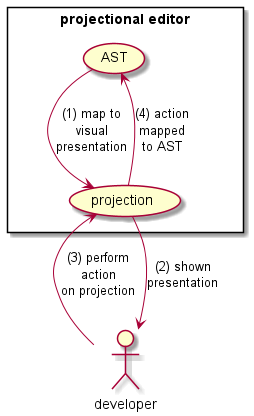
\includegraphics[width=0.35\textwidth]{Sections/images/projections.png}}
    \caption{Projectional editing loop. TODO: comparison with Parsing}
    \label{fig:projectionalEditing_loop}
\end{figure}

To perform the above two things have to be defined by language engineers: The Meta-Model and the editor.

The meta-model, analogous to the abstract syntax, describes the node concepts and connections used to build the hierarchical structure that is the AST.
This hierarchy can have references to nodes in other branches, so it is a graph although named a tree.
The AST is stored independently of the concrete syntax, often using a database, XML or a proprietary file format.
Rules of the meta-model, such as type systems or scoping rules, must also be described.

Projectional editors avoid the grammars and parsers that define the concrete and abstract syntax in a traditional text-based language.
In text-based languages, parsing transforms the concrete into the abstract.
In projectional editing, the abstract is transformed to concrete using a projection engine that uses projection rules.

Editors combine the projection rules and the gestures or actions to create a change request to the AST.
They are analogous to a concrete syntax.

One of these actions can be typing text. 
However, every string is recognized when entered.
Thus, there is no tokenizing.
Text enters into the templates defined by the editor, and a newly derived projection displays the adjusted underlying AST to the developer.

The projection uses graphical elements to represent the representation.
Although often appearing textual, each of the text elements are references to nodes in the AST.

Developers can only interact with the editor via the rigidly controlled code completion menus or gestures and actions.
She builds the AST directly from each interaction she has with the editor.

Nodes are instances of the concepts defined in the meta-model.
Each node has a unique id and points to its defining concept.
It is unambiguous.
References are first-class and defined by the id rather than resolved by name, as in parser-based languages.
Disambiguation happens at the time of input, as the developer chooses from limited legal inputs.

The separation of the abstract and concrete allows the language engineer to implement multiple projections of the same model, using different notations, each node of the AST taking having the design she envisions.
The pattern used for projection is similar to MVC, so multiple views of the program can be visible and updateable simultaneously.

Graphical modelling tools, for example for UML modelling, could be seen as specialized implementations of projectional editing.
These modelling tools do not store pictures of the UML diagrams and then parse them to create an AST.
Instead, they store the model, often with extra information about the visual layout, and the image of the UML is projected to the modeller to edit.
Projectional editing generalizes this approach to projecting any notation defined by the language engineer.

\subsection{History of Projectional Editing}

Here follows an incomplete and inconsistent history of projectional languages.

In the '70s and early '80s, researchers created several applications for research into the realm of structured editors.
Some examples were: MENTOR\cite{donzeau1980programming}, Incremental Programming Environment\cite{medina1981incremental}, GANDALF\cite{NotkinDavid1985TGp}, Cornell Program Synthesizer\cite{teitelbaum1981cornell}, and Synthesizer Generator\cite{reps2012synthesizer}.
These language-based program editors could force syntactically correct programs through the knowledge of the language.
These were the precursors to the modern projectional editors. 
They worked by providing templates for each abstract computational unit of the language.
First, one would choose the concept and then fill out the placeholders.

These tools were not good at editing textual notations, which led to a poor user experience.
When they attempted to fix this, for example, in the Synthesizer Generator, they reintroduced parsing to parts, which took away many advantages of the AST's direct editing.

In the late '90s and early '00s, the first forays into commercializing a more generalized version of structured editors, the projectional editors, began.
First, Intentional Domain Workbench, inspired by Charles Simonyi's 1995 essay ``The Death of Computer Languages, The Birth of Intentional Programming''\cite{simonyi1995death} the IDW was the product of the company Simonyi founded in 2002, Intentional Software. 
The Intentional Programming paradigm spotlighted the projectional editing domain, taking it out of the universities and into practice.
However, as it was a closed sourced and expensive product, thus not many papers were written about it.
In 2017, as part of an ``acquihire'', Microsoft bought Intentional Software for its employees and let the product die.

Inspired by a call to action for Language orientated programming\cite{dmitriev2004language} JetBrains embarked in 2004 on a mission to build a product to fulfil that ideal.  
Meta Programming System (MPS) was the outcome of that journey.   
Language engineers created the languages mbeddr, PEoPL, and Realaxy using the MPS platform.  
It currently has an active community of developers and projects both in academia and in the commercial world. 
We chose this tool to be the basis of our projectional editing experiments. 
We will talk about it at greater length in section \ref{section:MPS}.

The last decade has produced a few smaller projectional workbenches.
There are a few open-source, small team projectional projects.
In 2013 several projectional language workbenches joined MPS in the Language Workbench challenge\cite{erdweg2015evaluating}.
These included M\'as, a web-based projectional editor, which is no longer with us\cite{MasPostMortem}.
Whole Platform\cite{WholePlatformProductPage} is a projectional language workbench plugin for Eclipse.
Cedalion\cite{lorenz2011cedalion} provides another projectional IDE, specializing in internal DSLs.


More recently, there have been some new products that intersect the projectional domain.
Deuce\cite{hempel2018deuce} and Gentleman\cite{lafontant2020gentleman_SLR} are two recent projection editors that have recently emerged from academia.
The final two mentions in our incomplete history are a little out of left-field. 
Google's Blockly\cite{Blockly_ProductPage} is a tool for making structural editor languages, but only in a block format.
Blockly can create languages similar in style to the scratch language. 
Blueprint visual scripting, a part of the Unreal Engine, is a visual programming language for building concepts such as levels or game assets.
Examples of Blockly and Blueprint can be seen in figures \ref{fig:blockly} and \ref{fig:Blueprint} respectively.

\begin{figure}[H]
    \begin{subfigure}{.50\textwidth}
      \centering
      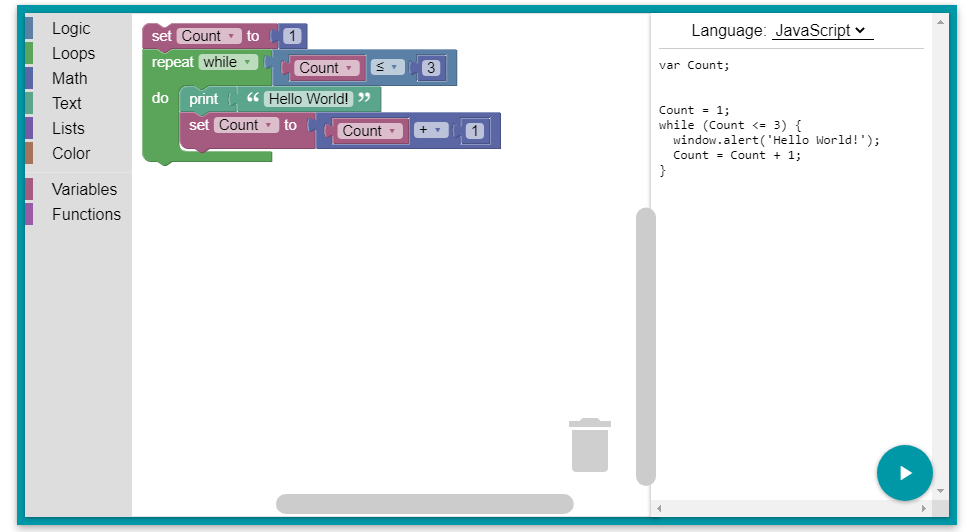
\includegraphics[width=.95\linewidth]{Sections/images/blockly.png}
      \caption{Blockly}
      \label{fig:blockly}
    \end{subfigure}%
    \begin{subfigure}{.50\textwidth}
      \centering
      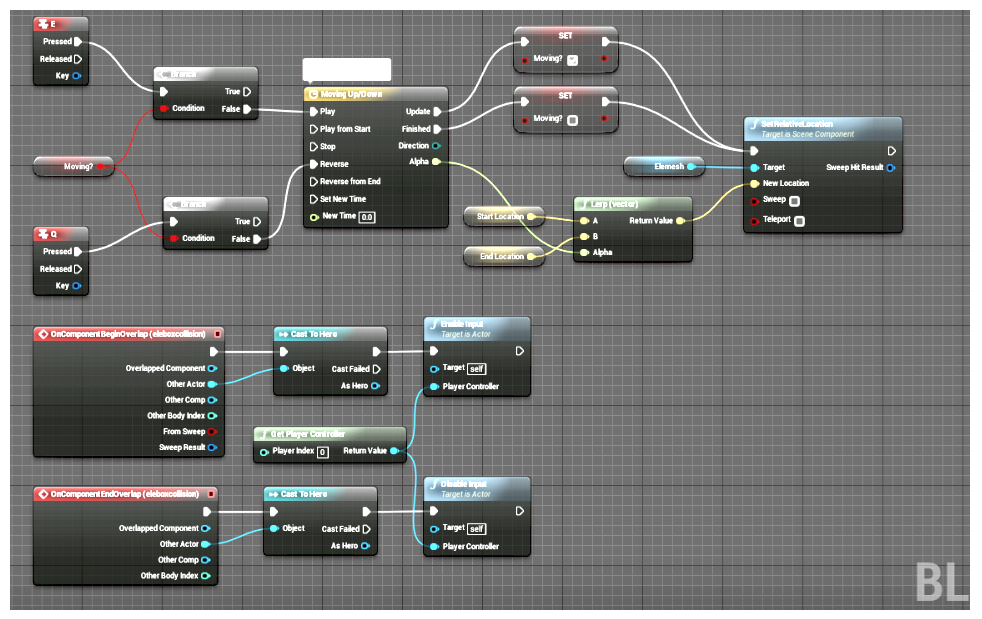
\includegraphics[width=.95\linewidth]{Sections/images/blueprint.png}
      \caption{Blueprint}
      \label{fig:Blueprint}
    \end{subfigure}
    \caption{Leftfield projectional editors}
    \label{fig:leftfield}
\end{figure}

\subsection{What Advantages Does Projectional Editing Bring?}
\label{section:projectional_advantages}

Projectional editing gives advantages both to the language engineer and the program developers.
There is a lot of crossover and repetition between papers written on projectional editing regarding the advantages it brings.
To that end, what follows is a synthesis of several papers as to the advantages that projectional editing claims.
Rather than attributing each advantage to each paper, we have made a reference table of papers proclaiming said advantage.
This is table \ref{table:Projectional_Advantages}.

\begin{table}[h]
    \begin{center}
        \begin{tabular}{ |l | c | l | } 
            \hline
            Advantage                   & \#& Paper(s)   \\
            \hline
            Exploratory programming     & 5 &\cite{klimevs2016domain,ratiu2017experiences,volter2010language,voelter2014towards,hosseinkord2021code}                                                                        \\
            Correctness-by-construction & 7 &\cite{voelter2013dsl,ratiu2019fasten,ratiu2012language,klimevs2016domain,berger2016efficiency,klimevs2016domain,vysoky2018ingrid}                                          \\
            Rich notation               & 22&\cite{pech2021jetbrains,voelter2014supporting,voelter2010language2,voelter2015using,voelter2010embedded,guttormsen2017consistent,voelter2010domain,wortmann2016domain,klimevs2016domain,voelter2013mbeddr,berger2016efficiency,simonyi2006intentional,voelter2016efficient,vysoky2018ingrid,pech2013jetbrains,volter2010language,voelter2014projecting,ratiu2018taming,voelter2015towards,voelter2014towards,simonyi1995death,voelter2019using} \\
            Mixed notation              & 8 &\cite{ratiu2017experiences,voelter2010language2,voelter2015using,voelter2010embedded,guttormsen2017consistent,volter2010language,voelter2014supporting,voelter2014towards}              \\
            Multiple views              & 9 &\cite{klimevs2016domain,voelter2016efficient,voelter2010language2,volter2010language,voelter2010embedded,voelter2010domain,vysoky2018ingrid,volter2010language,voelter2014supporting}   \\
            Language composition        & 23&\cite{voelter2013dsl, meacham2020adaptivevle, ratiu2019fasten, pavletic2013extensible,voelter2011language,guttormsen2017consistent,berger2016efficiency,voelter2016efficient,voelter2010embedded,ratiu2012implementing,volter2010language,voelter2010language2,voelter2012mbeddr,voelter2011product,voelter2013requirements,voelter2014supporting,voelter2014towards,voelter2015using,voelter2019using,simonyi1995death,vysoky2018ingrid,pech2013jetbrains,voelter2015towards} \\
            IDE functionality           & 3 &\cite{klimevs2016domain,voelter2010embedded,voelter2010language2}                                                                                                \\
            Language evolution          & 1 &\cite{schindler2016language} \\
            Ancillary data              & 5 &\cite{voelter2011product,voelter2013requirements,voelter2019using,volter2010language,voelter2010language2} \\
            \hline
        \end{tabular}
    \end{center}
    \caption{Papers describing advantages}
    \label{table:Projectional_Advantages}
\end{table}

 
\paragraph{Exploratory programming} As with their progenitors, syntax-directed editors, modern projectional editors help guide a developer unfamiliar with a language.
With their rigid syntax and predefined layout, the editors only allow editing within specific cells of the editor.
This template style means that the developer does not have to worry about the significance of spacing or indentation.
Minutiae of syntactic adornments, such as statement ending semi-colons or enclosing matched brackets, are also not interfering with her exploration of the language space.

When creating code, the editor only presents the developer with legal options within the current context.
As the projection is context-aware, with relevant actions and options suggested and irrelevant ones removed.
Thus, it is easier for the developer to explore what the language allows her to choose.
Intelligent code completion does not have to be limited to single nodes.
Inserting whole subtrees allows the developer to explore the larger structures of the language.

\paragraph{Correctness-by-construction} A projectional editor prevents her from writing syntactically incorrect code by controlling the interaction between the developer and the AST.
The whole class of syntactical errors is made impossible, with the developer relieved to think about special characters and layout.
Typing and scoping errors are removed by only allowing validly typed and scoped options for the developer.

The developer can only select statements that are legal in the context of the location within the AST.
Code does not have to be disambiguated, as this happens at the time of entry by the developer.
If multiple items share the same notation in the editor, the developer chooses the relevant item, thus resolving the ambiguity to what she means rather than what the parser thinks she means.

\paragraph{Rich notation} Constraints associated with textual parsing do not affect the choice of created projections. 
This freedom opens up diverse otherwise tricky or impossible to parse notations.
Examples include tabular, mathematical expressions and symbols, diagrams, trees, images, forms, prose, sub- and superscript.
Any visual form or shape that can map onto the AST can represent the program in an editor.

With these notations, one can better reflect the semantics of the program domain, which should aid comprehension.
Mathematics has a rich history of use of notation.
When writing a DSL for the Mathematics domain, the domain experts can interact with it in the centuries-old language of their domain.

Of course, the projections can also be projections of text.
Textual projections are often the appropriate projection type if the developer interacting with the language's domain expertise is parser-based languages.

\paragraph{Mixed notation} As no parsing is required and ambiguity is not an issue for the underlying AST, it is straightforward to combine different forms of rich notation.
With all notations working on the same editor infrastructure, embedding mathematic symbols within textual projections, within tables within graphical representations is a simple coding pattern.

\paragraph{Multiple views} With the AST being the stored artefact rather than the notation, projectional editing allows the language engineer to define multiple views on the same model optimised for different tasks.
In Software architecture, one presents different views to different stakeholders based on their interests.
Similarly, projectional editing can present experts with various domain expertise views on the model that reflect their needs.
A developer can switch between node projections within a larger projection to find the one that best suits their current task.

Because the architecture of a projectional editor follows the principles of model-view-controller, it is possible to have multiple simultaneous views of the model.
These multiple views allow the developer to update a projection optimised for writing and immediately see its effect in a projection optimised for understanding.

\paragraph{Language composition} Parser-based languages can support some modularization and composition, but a projectional editor allows easy and extensive modular language extension and composition.
This ability results from the disambiguation of the nodes of an AST at the time of entry.
If two items with the same syntax are available at the same place, the user will choose the one they require, and therefore the node has an explicitly chosen meaning.

The composition of independently developed languages does not suffer from the syntactic or keyword clashes they would in two grammar defined languages.
Because of the lack of ambiguity, every node referencing the concept that defines it, these languages, when put together, will not have structural or syntactic issues.

Language composition can involve extending an existing language or embedding other languages in a host language without modifying its definition.
The ease of composition and extensions allows building more significant languages out of smaller modules.

\paragraph{IDE functionality} Developers in mature languages are used to the functionality of mature IDEs.
These functionalities include syntax highlighting, intelligent code completion or suggestion, and static analysis for errors and validation.
As projectional languages store the AST rather than the concrete syntax, they require an IDE to edit.
Because of this, when a language engineer designs the language, she also has to design the IDE.

A projection always knows its context because it comes from the AST.
When the editor already knows the meaning of the node it represents, syntax highlighting is simple.
Knowing its context makes it much simpler to suggest intelligent code completions.

Always having a complete AST makes it much easier to validate scope, typing and other hard to implement code validators.

\paragraph{Language evolution} Parsing complicates the evolution of languages. 
For example, adding a new reserved word is difficult without breaking existing code.
Extending a language with new capabilities and syntax in projectional editing is simple.
If the change is syntactic, then the language engineer has to update an editor.
If there is a semantic change, then the language engineer can write a migration in the language to transform a node of one concept to a different type, and the developer would have to run that migration on their code.

\paragraph{Ancillary data} Data added to nodes can augment the AST.
This data is helpful for tasks such as documentation, requirements traceability and product line feature dependencies.

\subsection{What are the Disadvantages of Projectional Editing?}
\label{section:projectional_disadvantages}

Whilst fewer papers proclaim the disadvantages of projectional editing, we repeated the approach of the previous section.
Thus, we have synthesised the disadvantages from papers in the following sections and listed citations for these ideas in table \ref{table:Projectional_Disadvantages}.

We do not consider that the dearth of disadvantages discussed as evidence of projectional editing's superiority.
Our best guess is that those who do not find projectional editing useful do not write papers about it.

\begin{table}[h]
    \begin{center}
        \begin{tabular}{ |l | c | l | } 
            \hline
            Disadvantage               & \#& Paper(s)   \\
            \hline
            Low adoption               & 4 &\cite{vysoky2018ingrid,voelter2015using,voelter2015towards,voelter2014projecting} \\
            Unnatural user experience  & 11 &\cite{vysoky2018ingrid,voelter2015towards,voelter2014towards,voelter2012mbeddr,voelter2014projecting,berger2016efficiency,voelter2016efficient,voelter2010embedded,voelter2010language2,schindler2016language,voelter2014supporting} \\
            Ambiguous syntax           & 1 &\cite{guttormsen2017consistent} \\
            Inflexibility              & 2 &\cite{voelter2014towards,voelter2014supporting} \\
            lack of integration with text ecosystem & 5 &\cite{voelter2012mbeddr,voelter2014towards,voelter2012mbeddr,voelter2014projecting,voelter2014supporting} \\
            Learning curve             & 5 &\cite{voelter2010language2,pech2013jetbrains,voelter2012mbeddr,voelter2014towards,voelter2015using,prinz2021teaching} \\
            Vendor lock\-in            & 2 &\cite{voelter2010embedded,voelter2010language2,tomassetti2020reflections} \\
            \hline
        \end{tabular}
    \end{center}
    \caption{Papers describing projectional editing disadvantages}
    \label{table:Projectional_Disadvantages}
\end{table}

\paragraph{Lack of adoption} The ideas that proceeded projectional editing - the structured or syntax-directed editor - have been around since the early 1970s yet have failed to be adopted widely.
This argument is a bit of a tautological one, as the low adoption is perhaps an outcome of the other disadvantages of projectional editing.
However, low adoption can lead to a self-reinforcing process, where lack of adoption prevents further adoption.

\paragraph{Inconvenient or unnatural editing} Early attempts at projectional editing presented an inconvenient and unnatural user experience when coding.
These usability challenges, exemplified by the tedious manner of entering code as per the tree's order, compare poorly to parser-based languages.

This lousy reputation continues, despite massive improvements in projectional editors.
Whilst there is no debate that projectional editing feels different, some question whether this inconvenience is an intrinsic property or a result of developers, through years of experience, being used to text-based programming.

Modern projectional editors, when using a textual projection, face an ``uncanny valley'' issue.
Whilst trying to simulate a text editor, the developers start to expect all of the functionality of the text-based IDEs.
This expectation is an especially weak trait regarding granularity and restrictions of cursor movement, insertion, deletion, selection, copy and paste, and other interactions with the text.

\paragraph{Ambiguous syntax} One of the selling points of projectional editing, especially concerning language composition, is that there can be no ambiguous syntax.
While this may be true for the AST, it is not so for the developer who reads this code on the screen.
If one combined Drools and Basic rather than Java, the developer might become confused about which language the ``Then'' keyword refers to when she read it.
Thus writing ambiguity is replaced by reading ambiguity.

\paragraph{Inflexibility} A developer using a projectional editor has no flexibility in code layout. They may feel they require this for enhanced readability.
The flexibility of the layout is entirely in the hands of the language engineer when she determines the projection rules.

\paragraph{Integration with the text based world} Projectional editors do not store the definition of the program in the form of a plain-text implementation in the concrete syntax.
Instead, the AST is stored and serialized in a non-human readable format, such as XML.

This different format of program storage leads to an issue with integration with the text-based ecosystem.
This ecosystem is extensive, as text-based coding has been popular since the 60s.
Two notable examples are text diffing, especially where branch merging is concerned and code sharing.
The diffing issue within projectional editing tools is solved.
However, as code-bases often span multiple programming languages and tools, the difficulty of integrating projectional diffing into the software development workflows is still a real problem.

Textual source code can be shared simply by email or on websites. 
This sharing, however, is not easy with projectional code.

\paragraph{Learning curve} For the language engineer, the necessity to develop an editor with a good user experience is much harder work than defining a grammar for a parsed language.
The learning curve for the language engineer is significant, as, by default, she has to think also of the IDE development.

For the developer, especially one with an extensive text-based experience, the different editing style takes some getting used to.

\paragraph{Vendor lock-in} The nature of projectional editing is that what one edits is a projection of the AST, and therefore an IDE is needed to do the projecting and language definition.
The fear of getting locked into a specific concept implementation can negatively impact evaluations of projectional editing by organisations.
To be able to use previously developed languages would require using the same toolset.
Changing to a different toolset for language design would require a significant re-skilling effort.